\documentclass{standalone}
\usepackage{tikz}
\usetikzlibrary{patterns, positioning}


\begin{document}
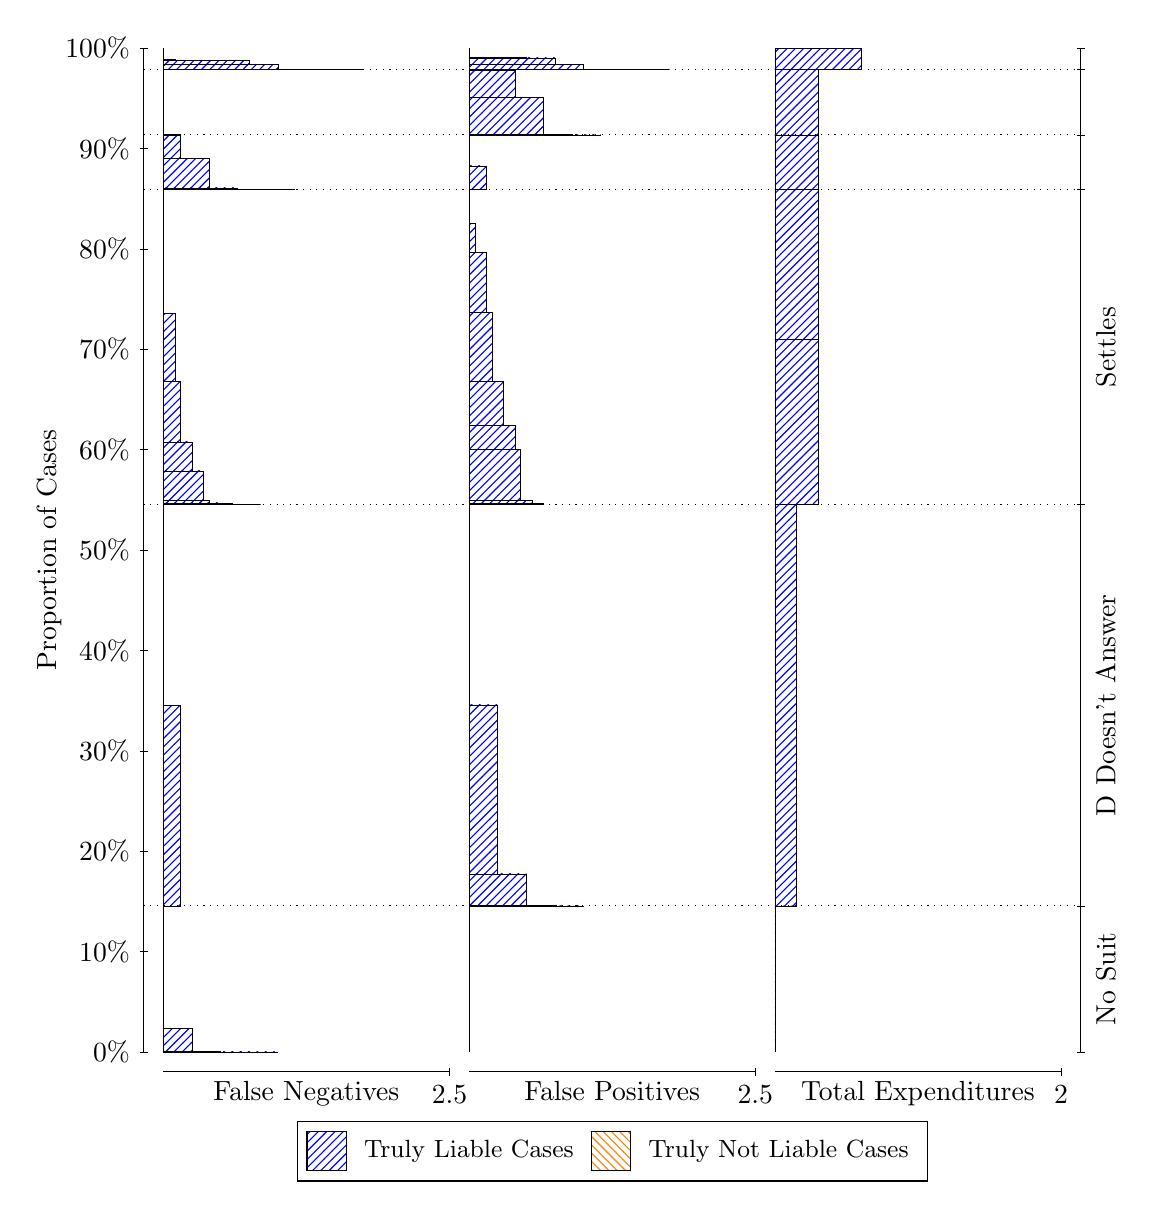
\begin{tikzpicture}
\draw[black, very thin] (1.5,1.75) -- (1.5,14.5);
\node[rotate=90, text=black, anchor=center] at (0.3, 8.125) {Proportion of Cases};
\draw[black, very thin] (1.45,1.75) -- (1.55,1.75);
\node[text=black, anchor=east] at (1.45, 1.75) {0\%};
\draw[black, very thin] (1.45,3.025) -- (1.55,3.025);
\node[text=black, anchor=east] at (1.45, 3.025) {10\%};
\draw[black, very thin] (1.45,4.3) -- (1.55,4.3);
\node[text=black, anchor=east] at (1.45, 4.3) {20\%};
\draw[black, very thin] (1.45,5.575) -- (1.55,5.575);
\node[text=black, anchor=east] at (1.45, 5.575) {30\%};
\draw[black, very thin] (1.45,6.85) -- (1.55,6.85);
\node[text=black, anchor=east] at (1.45, 6.85) {40\%};
\draw[black, very thin] (1.45,8.125) -- (1.55,8.125);
\node[text=black, anchor=east] at (1.45, 8.125) {50\%};
\draw[black, very thin] (1.45,9.4) -- (1.55,9.4);
\node[text=black, anchor=east] at (1.45, 9.4) {60\%};
\draw[black, very thin] (1.45,10.675) -- (1.55,10.675);
\node[text=black, anchor=east] at (1.45, 10.675) {70\%};
\draw[black, very thin] (1.45,11.95) -- (1.55,11.95);
\node[text=black, anchor=east] at (1.45, 11.95) {80\%};
\draw[black, very thin] (1.45,13.225) -- (1.55,13.225);
\node[text=black, anchor=east] at (1.45, 13.225) {90\%};
\draw[black, very thin] (1.45,14.5) -- (1.55,14.5);
\node[text=black, anchor=east] at (1.45, 14.5) {100\%};

\draw[black, very thin] (13.4,1.75) -- (13.4,14.5);
\draw[black, very thin] (13.35,1.75) -- (13.45,1.75);
\node[anchor=west] at (13.35, 1.75) {};
\draw[black, very thin] (13.35,3.6057) -- (13.45,3.6057);
\node[anchor=west] at (13.35, 3.6057) {};
\draw[black, very thin] (13.35,8.7036) -- (13.45,8.7036);
\node[anchor=west] at (13.35, 8.7036) {};
\draw[black, very thin] (13.35,12.7) -- (13.45,12.7);
\node[anchor=west] at (13.35, 12.7) {};
\draw[black, very thin] (13.35,13.397) -- (13.45,13.397);
\node[anchor=west] at (13.35, 13.397) {};
\draw[black, very thin] (13.35,14.227) -- (13.45,14.227);
\node[anchor=west] at (13.35, 14.227) {};
\draw[black, very thin] (13.35,14.5) -- (13.45,14.5);
\node[anchor=west] at (13.35, 14.5) {};

\draw[black, very thin, pattern color=blue, pattern=north east lines] (1.75,1.75) rectangle (3.2033,1.75);
\draw[black, very thin, pattern color=blue, pattern=north east lines] (1.75,1.75) rectangle (2.84,1.75);
\draw[black, very thin, pattern color=blue, pattern=north east lines] (1.75,1.75) rectangle (2.4767,1.7526);
\draw[black, very thin, pattern color=blue, pattern=north east lines] (1.75,1.7526) rectangle (2.1133,2.0538);
\draw[black, very thin, pattern color=orange, pattern=north west lines] (1.75,2.0538) rectangle (1.75,2.0538);
\draw[black, very thin, pattern color=blue, pattern=north east lines] (1.75,2.0538) rectangle (1.75,3.6057);
\draw[black, very thin, pattern color=blue, pattern=north east lines] (1.75,3.6057) rectangle (1.968,6.1515);
\draw[black, very thin, pattern color=orange, pattern=north west lines] (1.75,6.1515) rectangle (1.75,6.1515);
\draw[black, very thin, pattern color=blue, pattern=north east lines] (1.75,6.1515) rectangle (1.75,8.7036);
\draw[black, very thin, pattern color=blue, pattern=north east lines] (1.75,8.7036) rectangle (2.9853,8.7036);
\draw[black, very thin, pattern color=blue, pattern=north east lines] (1.75,8.7036) rectangle (2.84,8.7036);
\draw[black, very thin, pattern color=blue, pattern=north east lines] (1.75,8.7036) rectangle (2.6947,8.7037);
\draw[black, very thin, pattern color=blue, pattern=north east lines] (1.75,8.7037) rectangle (2.622,8.7146);
\draw[black, very thin, pattern color=blue, pattern=north east lines] (1.75,8.7146) rectangle (2.4767,8.7244);
\draw[black, very thin, pattern color=blue, pattern=north east lines] (1.75,8.7244) rectangle (2.3313,8.7577);
\draw[black, very thin, pattern color=blue, pattern=north east lines] (1.75,8.7577) rectangle (2.2587,9.131);
\draw[black, very thin, pattern color=blue, pattern=north east lines] (1.75,9.131) rectangle (2.1133,9.4977);
\draw[black, very thin, pattern color=blue, pattern=north east lines] (1.75,9.4977) rectangle (1.968,10.265);
\draw[black, very thin, pattern color=blue, pattern=north east lines] (1.75,10.265) rectangle (1.8953,11.134);
\draw[black, very thin, pattern color=orange, pattern=north west lines] (1.75,11.134) rectangle (1.75,11.134);
\draw[black, very thin, pattern color=blue, pattern=north east lines] (1.75,11.134) rectangle (1.75,12.7);
\draw[black, very thin, pattern color=blue, pattern=north east lines] (1.75,12.7) rectangle (3.4213,12.7);
\draw[black, very thin, pattern color=blue, pattern=north east lines] (1.75,12.7) rectangle (3.058,12.7);
\draw[black, very thin, pattern color=blue, pattern=north east lines] (1.75,12.7) rectangle (2.6947,12.723);
\draw[black, very thin, pattern color=blue, pattern=north east lines] (1.75,12.723) rectangle (2.3313,13.096);
\draw[black, very thin, pattern color=blue, pattern=north east lines] (1.75,13.096) rectangle (1.968,13.397);
\draw[black, very thin, pattern color=orange, pattern=north west lines] (1.75,13.397) rectangle (1.75,13.397);
\draw[black, very thin, pattern color=blue, pattern=north east lines] (1.75,13.397) rectangle (1.968,13.401);
\draw[black, very thin, pattern color=orange, pattern=north west lines] (1.75,13.401) rectangle (1.75,13.401);
\draw[black, very thin, pattern color=blue, pattern=north east lines] (1.75,13.401) rectangle (1.75,14.227);
\draw[black, very thin, pattern color=blue, pattern=north east lines] (1.75,14.227) rectangle (4.2933,14.227);
\draw[black, very thin, pattern color=blue, pattern=north east lines] (1.75,14.227) rectangle (3.93,14.227);
\draw[black, very thin, pattern color=blue, pattern=north east lines] (1.75,14.227) rectangle (3.5667,14.23);
\draw[black, very thin, pattern color=blue, pattern=north east lines] (1.75,14.23) rectangle (3.2033,14.288);
\draw[black, very thin, pattern color=blue, pattern=north east lines] (1.75,14.288) rectangle (2.84,14.343);
\draw[black, very thin, pattern color=blue, pattern=north east lines] (1.75,14.343) rectangle (2.622,14.343);
\draw[black, very thin, pattern color=blue, pattern=north east lines] (1.75,14.343) rectangle (2.4767,14.345);
\draw[black, very thin, pattern color=blue, pattern=north east lines] (1.75,14.345) rectangle (2.2587,14.345);
\draw[black, very thin, pattern color=blue, pattern=north east lines] (1.75,14.345) rectangle (2.2587,14.345);
\draw[black, very thin, pattern color=blue, pattern=north east lines] (1.75,14.345) rectangle (2.1133,14.345);
\draw[black, very thin, pattern color=blue, pattern=north east lines] (1.75,14.345) rectangle (1.8953,14.346);
\draw[black, very thin, pattern color=blue, pattern=north east lines] (1.75,14.346) rectangle (1.8953,14.351);
\draw[black, very thin, pattern color=orange, pattern=north west lines] (1.75,14.351) rectangle (1.75,14.351);
\draw[black, very thin, pattern color=blue, pattern=north east lines] (1.75,14.351) rectangle (1.75,14.5);
\draw[black, very thin, pattern color=orange, pattern=north west lines] (5.6333,1.75) rectangle (5.6333,1.75);
\draw[black, very thin, pattern color=blue, pattern=north east lines] (5.6333,1.75) rectangle (5.6333,3.6057);
\draw[black, very thin, pattern color=orange, pattern=north west lines] (5.6333,3.6057) rectangle (7.0867,3.6057);
\draw[black, very thin, pattern color=blue, pattern=north east lines] (5.6333,3.6057) rectangle (7.0867,3.6057);
\draw[black, very thin, pattern color=blue, pattern=north east lines] (5.6333,3.6057) rectangle (6.7233,3.6087);
\draw[black, very thin, pattern color=blue, pattern=north east lines] (5.6333,3.6087) rectangle (6.36,4.0129);
\draw[black, very thin, pattern color=blue, pattern=north east lines] (5.6333,4.0129) rectangle (5.9967,6.1578);
\draw[black, very thin, pattern color=blue, pattern=north east lines] (5.6333,6.1578) rectangle (5.6333,8.7036);
\draw[black, very thin, pattern color=orange, pattern=north west lines] (5.6333,8.7036) rectangle (6.578,8.7036);
\draw[black, very thin, pattern color=blue, pattern=north east lines] (5.6333,8.7036) rectangle (6.578,8.7143);
\draw[black, very thin, pattern color=orange, pattern=north west lines] (5.6333,8.7143) rectangle (6.4327,8.7143);
\draw[black, very thin, pattern color=blue, pattern=north east lines] (5.6333,8.7143) rectangle (6.4327,8.7535);
\draw[black, very thin, pattern color=orange, pattern=north west lines] (5.6333,8.7535) rectangle (6.2873,8.7535);
\draw[black, very thin, pattern color=blue, pattern=north east lines] (5.6333,8.7535) rectangle (6.2873,9.3984);
\draw[black, very thin, pattern color=blue, pattern=north east lines] (5.6333,9.3984) rectangle (6.2147,9.7092);
\draw[black, very thin, pattern color=blue, pattern=north east lines] (5.6333,9.7092) rectangle (6.0693,10.27);
\draw[black, very thin, pattern color=blue, pattern=north east lines] (5.6333,10.27) rectangle (5.924,11.139);
\draw[black, very thin, pattern color=blue, pattern=north east lines] (5.6333,11.139) rectangle (5.8513,11.906);
\draw[black, very thin, pattern color=blue, pattern=north east lines] (5.6333,11.906) rectangle (5.706,12.273);
\draw[black, very thin, pattern color=blue, pattern=north east lines] (5.6333,12.273) rectangle (5.6333,12.7);
\draw[black, very thin, pattern color=orange, pattern=north west lines] (5.6333,12.7) rectangle (5.8513,12.7);
\draw[black, very thin, pattern color=blue, pattern=north east lines] (5.6333,12.7) rectangle (5.8513,13.002);
\draw[black, very thin, pattern color=blue, pattern=north east lines] (5.6333,13.002) rectangle (5.6333,13.397);
\draw[black, very thin, pattern color=orange, pattern=north west lines] (5.6333,13.397) rectangle (7.3047,13.397);
\draw[black, very thin, pattern color=blue, pattern=north east lines] (5.6333,13.397) rectangle (7.3047,13.397);
\draw[black, very thin, pattern color=blue, pattern=north east lines] (5.6333,13.397) rectangle (6.9413,13.408);
\draw[black, very thin, pattern color=blue, pattern=north east lines] (5.6333,13.408) rectangle (6.578,13.875);
\draw[black, very thin, pattern color=blue, pattern=north east lines] (5.6333,13.875) rectangle (6.2147,14.223);
\draw[black, very thin, pattern color=blue, pattern=north east lines] (5.6333,14.223) rectangle (5.8513,14.227);
\draw[black, very thin, pattern color=orange, pattern=north west lines] (5.6333,14.227) rectangle (8.1767,14.227);
\draw[black, very thin, pattern color=blue, pattern=north east lines] (5.6333,14.227) rectangle (8.1767,14.227);
\draw[black, very thin, pattern color=orange, pattern=north west lines] (5.6333,14.227) rectangle (7.8133,14.227);
\draw[black, very thin, pattern color=blue, pattern=north east lines] (5.6333,14.227) rectangle (7.8133,14.227);
\draw[black, very thin, pattern color=orange, pattern=north west lines] (5.6333,14.227) rectangle (7.45,14.227);
\draw[black, very thin, pattern color=blue, pattern=north east lines] (5.6333,14.227) rectangle (7.45,14.233);
\draw[black, very thin, pattern color=orange, pattern=north west lines] (5.6333,14.233) rectangle (7.0867,14.233);
\draw[black, very thin, pattern color=blue, pattern=north east lines] (5.6333,14.233) rectangle (7.0867,14.295);
\draw[black, very thin, pattern color=blue, pattern=north east lines] (5.6333,14.295) rectangle (6.7233,14.376);
\draw[black, very thin, pattern color=blue, pattern=north east lines] (5.6333,14.376) rectangle (6.36,14.381);
\draw[black, very thin, pattern color=orange, pattern=north west lines] (5.6333,14.381) rectangle (6.142,14.381);
\draw[black, very thin, pattern color=blue, pattern=north east lines] (5.6333,14.381) rectangle (6.142,14.381);
\draw[black, very thin, pattern color=blue, pattern=north east lines] (5.6333,14.381) rectangle (5.9967,14.381);
\draw[black, very thin, pattern color=orange, pattern=north west lines] (5.6333,14.381) rectangle (5.7787,14.381);
\draw[black, very thin, pattern color=blue, pattern=north east lines] (5.6333,14.381) rectangle (5.7787,14.383);
\draw[black, very thin, pattern color=orange, pattern=north west lines] (5.6333,14.383) rectangle (5.6333,14.383);
\draw[black, very thin, pattern color=blue, pattern=north east lines] (5.6333,14.383) rectangle (5.6333,14.5);
\draw[black, very thin, pattern color=orange, pattern=north west lines] (9.5167,1.75) rectangle (9.5167,1.75);
\draw[black, very thin, pattern color=blue, pattern=north east lines] (9.5167,1.75) rectangle (9.5167,3.6057);
\draw[black, very thin, pattern color=orange, pattern=north west lines] (9.5167,3.6057) rectangle (9.7892,3.6057);
\draw[black, very thin, pattern color=blue, pattern=north east lines] (9.5167,3.6057) rectangle (9.7892,8.7036);
\draw[black, very thin, pattern color=orange, pattern=north west lines] (9.5167,8.7036) rectangle (10.062,8.7036);
\draw[black, very thin, pattern color=blue, pattern=north east lines] (9.5167,8.7036) rectangle (10.062,10.802);
\draw[black, very thin, pattern color=orange, pattern=north west lines] (9.5167,10.802) rectangle (10.062,10.802);
\draw[black, very thin, pattern color=blue, pattern=north east lines] (9.5167,10.802) rectangle (10.062,12.7);
\draw[black, very thin, pattern color=orange, pattern=north west lines] (9.5167,12.7) rectangle (10.062,12.7);
\draw[black, very thin, pattern color=blue, pattern=north east lines] (9.5167,12.7) rectangle (10.062,13.397);
\draw[black, very thin, pattern color=orange, pattern=north west lines] (9.5167,13.397) rectangle (10.062,13.397);
\draw[black, very thin, pattern color=blue, pattern=north east lines] (9.5167,13.397) rectangle (10.062,14.227);
\draw[black, very thin, pattern color=orange, pattern=north west lines] (9.5167,14.227) rectangle (10.607,14.227);
\draw[black, very thin, pattern color=blue, pattern=north east lines] (9.5167,14.227) rectangle (10.607,14.5);
\draw[black, dotted] (1.5,3.6057) -- (13.4,3.6057);
\draw[black, dotted] (1.5,8.7036) -- (13.4,8.7036);
\draw[black, dotted] (1.5,12.7) -- (13.4,12.7);
\draw[black, dotted] (1.5,13.397) -- (13.4,13.397);
\draw[black, dotted] (1.5,14.227) -- (13.4,14.227);
\draw[black, very thin] (1.75,1.5) -- (5.3833,1.5);
\node[text=black, anchor=north] at (3.5667, 1.5) {False Negatives};
\draw[black, very thin] (5.3833,1.45) -- (5.3833,1.55);
\node[text=black, anchor=north] at (5.3833, 1.45) {2.5};

\draw[black, very thin] (5.6333,1.5) -- (9.2667,1.5);
\node[text=black, anchor=north] at (7.45, 1.5) {False Positives};
\draw[black, very thin] (9.2667,1.45) -- (9.2667,1.55);
\node[text=black, anchor=north] at (9.2667, 1.45) {2.5};

\draw[black, very thin] (9.5167,1.5) -- (13.15,1.5);
\node[text=black, anchor=north] at (11.333, 1.5) {Total Expenditures};
\draw[black, very thin] (13.15,1.45) -- (13.15,1.55);
\node[text=black, anchor=north] at (13.15, 1.45) {2};

\node[text=black, centered, rotate=90] at (13.72, 2.6778) {No Suit};
\node[text=black, centered, rotate=90] at (13.72, 6.1547) {D Doesn't Answer};
\node[text=black, centered, rotate=90] at (13.72, 10.702) {Settles};




\draw (7.449999999999999,1.5) node[draw=none] (baseCoordinate) {};
\begin{scope}[align=center]
        \matrix[scale=0.5, draw=black, below=0.5cm of baseCoordinate, nodes={draw}, column sep=0.1cm]{
            \node[rectangle, draw, minimum width=0.5cm, minimum height=0.5cm, pattern color=blue, pattern=north east lines] {}; &
            \node[draw=none, font=\small, text=black] (B) {Truly Liable Cases}; &
            \node[rectangle, draw, minimum width=0.5cm, minimum height=0.5cm, pattern color=orange, pattern=north west lines] {}; &
            \node[draw=none, font=\small, text=black] (B) {Truly Not Liable Cases}; \\
            };
\end{scope}

\end{tikzpicture}
\end{document}